\section{Stability and Equilibrium of $N=100$ System}
\label{sec:StabilityAndEquilibrium}
From the histograms in \figref{fig:histograms_RK4_diff_time_step}, it is expected that the extend of the cluster will vary with time. 
In the histograms of \figref{fig:StabilityEquilibriumHistogram}, the final position of 100 uniformly distributed particles with Gaussian distributed masses, as previous, is computed with the fourth order Runge-Kutta method after $1\tau_{crunch}$ and $4\tau_{crunch}$ with the same step length, $dt = 10^{-3} \tau_{crunch}$. 
Similar histograms are made for the final position after $0.5\tau_{crunch}$, $1.5\tau_{crunch}$, $2\tau_{crunch}$, $2.5\tau_{crunch}$, $3\tau_{crunch}$, as well. 
However, these histograms are not explicitly shown in this work. 
\begin{figure}[H]
\centering
\begin{minipage}{.5\textwidth}
  \centering
  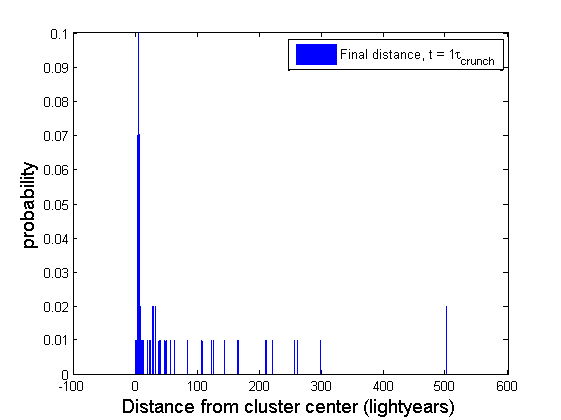
\includegraphics[width=1\linewidth]{Figures/stability/RK4_stability_1t.png}
\end{minipage}%
\begin{minipage}{.5\textwidth}
  \centering
  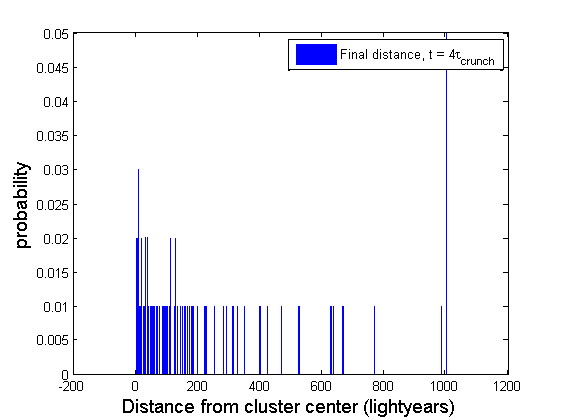
\includegraphics[width=1\linewidth]{Figures/stability/RK4_stability_4t_2_zoom.png}
\end{minipage}
\caption{
Final radial position of 100 particles after $1\tau_{crunch}$ and $4\tau_{crunch}$ with a step length of $10^{-3} \tau_{crunch}$.
The "high" densities at 500 ly and 1000 ly represent particles further away from the cluster center than 500 ly or 1000 ly, respectively.
The extend of the cluster is here defined as the first particle than has a distance of 100 ly to the next particle further from the cluster center. 
Hence after $1\tau_{crunch}$, the extend of the cluster is 166 ly, whilst after $4\tau_{crunch}$, the cluster extend is 525 ly.
}
\label{fig:StabilityEquilibriumHistogram}
\end{figure}
The knowledge of the cluster extend as a function of time gained from \figref{fig:StabilityEquilibriumHistogram} is plotted in the figure below. 
The plotted data show reaching of an equilibrium after approximately $2\tau_{crunch}$.
Another argument for reaching the equilibrium after about $2\tau_{crunch}$ is the number of particles within a sphere of radius of $10$ ly, which is inspired by the great density of particles within this sphere compared to density outside this sphere after $10^7$ years, shown in the histograms of \figref{fig:histograms_RK4_diff_time_step}. 

%\begin{figure}[H]
%\centering
%	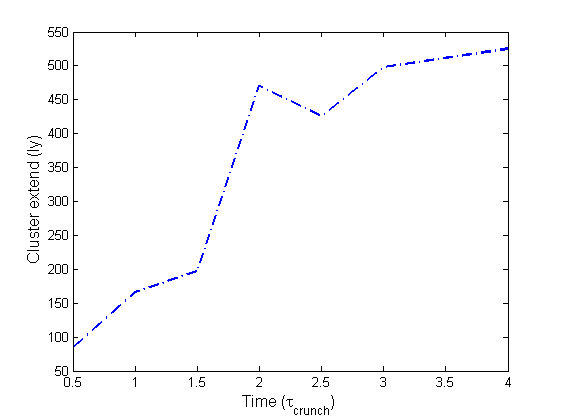
\includegraphics[width=0.6\linewidth]{Figures/Stability_cluster_extend_time_dependence.png}
%\caption{
%Plot of the cluster extend as a function of the final time. The cluster extend is determined from histograms similar to the ones shown in \figref{fig:StabilityEquilibriumHistogram}.
%}
%\label{fig:StailityEquilibriumLineGraph}
%\end{figure}
\begin{minipage}{\textwidth}
  \begin{minipage}[c]{.5\textwidth}
    \centering
    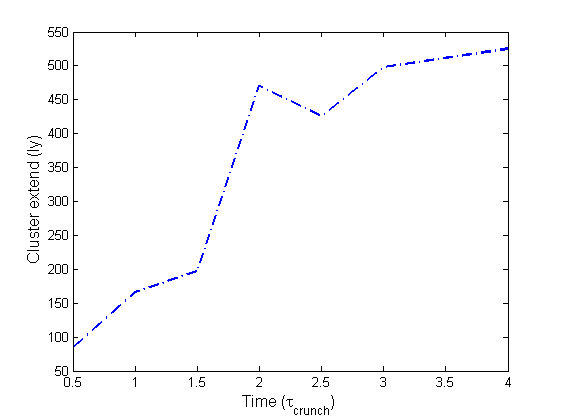
\includegraphics[width=1\linewidth]{Figures/Stability_cluster_extend_time_dependence.png}
    \captionof{figure}{Plot of the cluster extend as a function of the final time. The cluster extend is determined from histograms similar to the ones shown in \figref{fig:StabilityEquilibriumHistogram}.}
    \label{fig:StailityEquilibriumLineGraph}
  \end{minipage}
  \hfill
  \begin{minipage}[c]{.5\textwidth}
    \centering
    \begin{tabular}{|c|c|}\hline
      	Time [$\tau_{crunch}$] & \# particles \\ \hline
        0.5 & 31 \\
        1 & 62 \\
        1.5 & 38 \\
        2 & 23 \\
        2.5 & 17 \\
        3 & 6 \\ 
        4 & 12
        \\ \hline
      \end{tabular}
      \captionof{table}{Number of particles within a sphere of radius $10$ ly after various times.}
    \end{minipage}
  \end{minipage}
\end{document}